The probability of the hyper-parameters of a GP as defined above and given covariance function structure $\mathbf{K}$ is:
\begin{equation}
\label{eq:hyperProbability}
P(\bm{\theta} \mid \mathbf{D,K}) = \frac{P(\mathbf{D} \mid \bm{\theta}, \mathbf{K})P(\bm{\theta} \mid  \mathbf{K})}{P(\mathbf{D} \mid \mathbf{K})}.
\end{equation}
Let the $\mathbf{K}$ be the sum of a smoothing and a white noise (WN) kernel. For this case, Neal~\citeyearpar{neal1997monte} suggested the problem of outliers in data as a use-case for a hierarchical Bayesian treatment of Gaussian processes\footnote{In \citep{neal1997monte} the sum of an SE plus a constant kernel is used. We keep the WN kernel for illustrative purposes.}. The work suggests a hierarchical system of hyper-parameterization. Here, we draw hyper-parameters from a $\Gamma$ distributions:
\begin{equation}
\label{eq:hyper-ell}
\ell^{(t)} \sim \Gamma(\alpha_1,\beta_1),\;\sigma^{(t)} \sim \Gamma(\alpha_2,\beta_2)
\end{equation} 
and in turn sample the $\alpha$ and $\beta$ from $\Gamma$ distributions as well:
\begin{equation}
\label{eq:hyper-alpha}
\alpha_1^{(t)} \sim \Gamma(\alpha^1_{\alpha},\beta^1_{ \alpha } ),\; \alpha_2^{(t)} \sim \Gamma(\alpha^2_{\alpha},\beta^2_{\alpha}),\cdots
\end{equation}
% the input below will be empty, if we're in the paper. For my thesis, it will contain a causal network of the hyper-parameters.
One can represent this kind of model using \gpmem\ (Listing \ref{alg:gphierarch}).
Neal provides a custom inference algorithm setting and evaluates it using the following synthetic data problem. Let $f$ be the underlying function that generates the data:
\begin{equation}
f(x) =  0.3 + 0.4 x + 0.5 \sin(2.7x) + \frac{1.1}{(1+ x^2)} + \eta \;\;\; with\;\;\eta \sim \mathcal{N}(0,\sigma)
\end{equation}
We synthetically generate outliers by setting $\sigma = 0.1$ in $95\%$ of the cases and to $\sigma = 1$ in the remaining cases. \gpmem\  can capture the true underlying function within only 100 MH steps on the hyper-parameters to get a good approximation for their posterior (see Fig. \ref{fig:neal}). Note that Neal devises an additional noise model and performs a large number of Hybrid-Monte Carlo and Gibbs steps.  
\begin{comment}
 


\begin{figure}
        \centering
         %add desired spacing between images, e. g. ~, \quad, \qquad, \hfill etc.
          %(or a blank line to force the subfigure onto a new line)
        \begin{subfigure}[b]{0.24\textwidth} \centering
                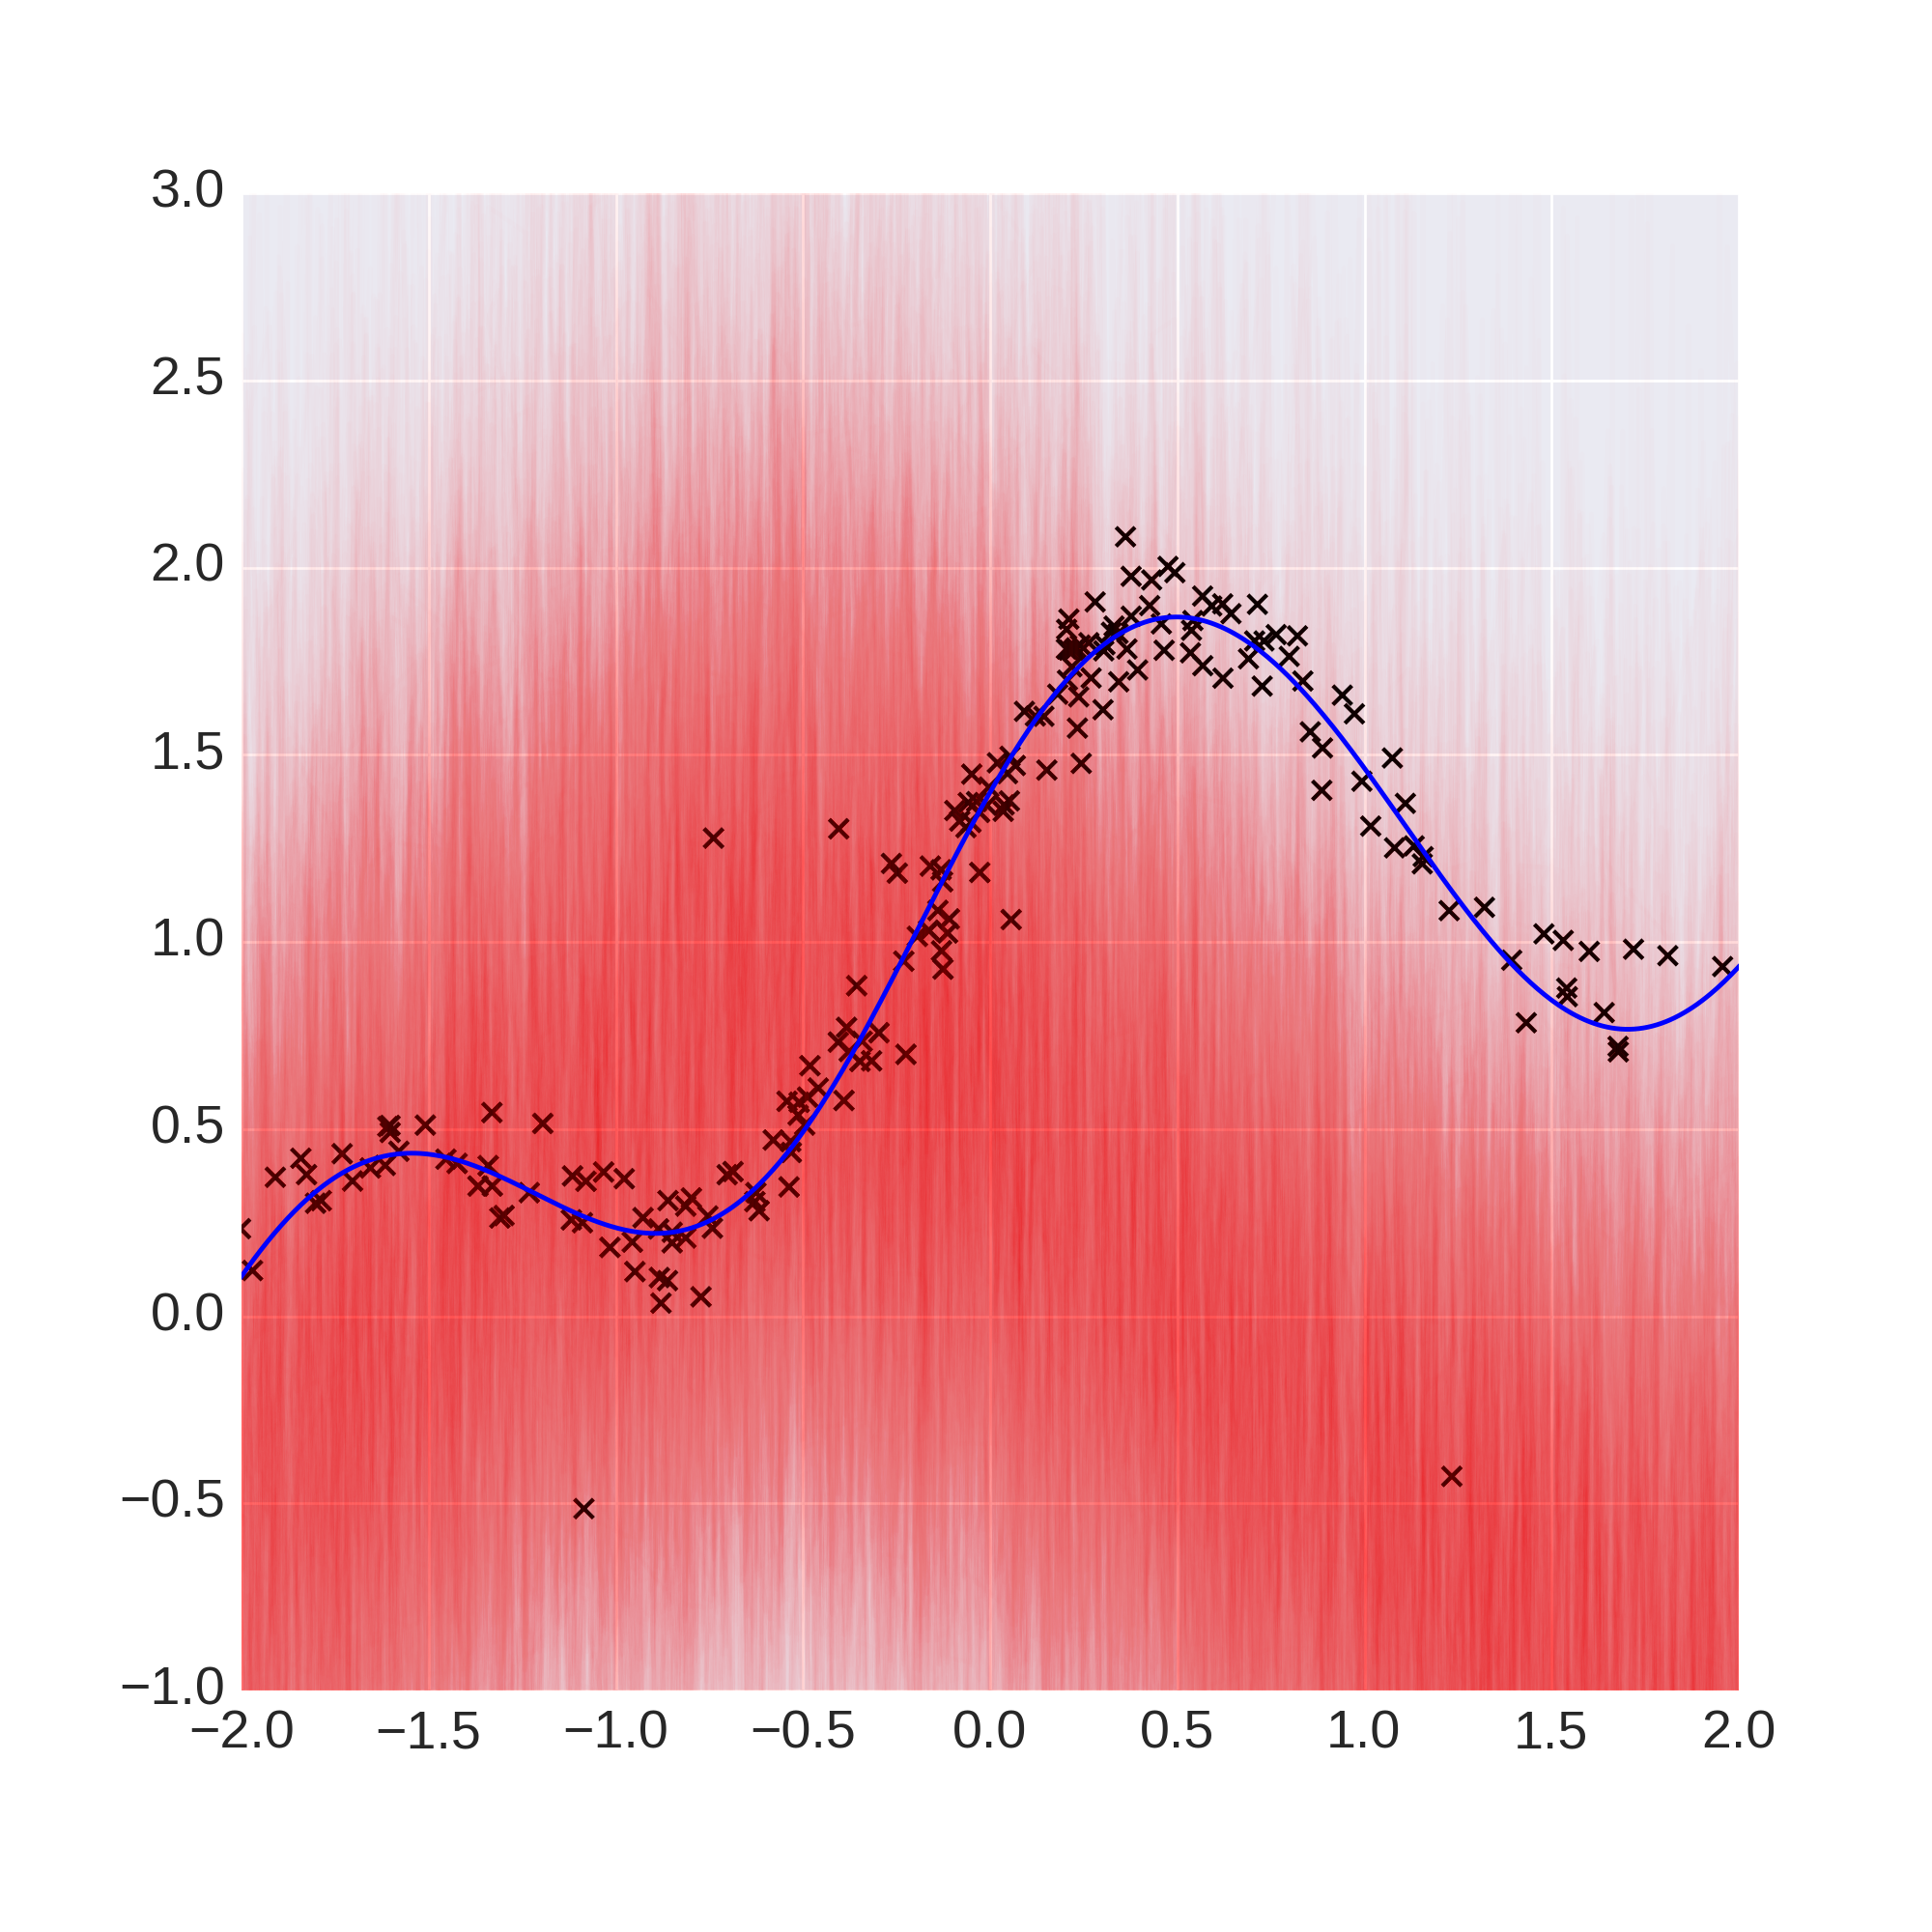
\includegraphics[height=3.9cm]{figs/neal_se_2final.png}
                        \put(-76,24){\color{green} \thicklines \circle{10}}
			\put(-28,26){\color{green} \thicklines  \circle{10}}
			\put(-70,63){\color{green} \thicklines  \circle{10}}
	
                \caption{Observed}
                \label{fig:NealAO}
        \end{subfigure}
         %add desired spacing between images, e. g. ~, \quad, \qquad, \hfill etc.
          %(or a blank line to force the subfigure onto a new line)
        \begin{subfigure}[b]{0.24\textwidth} \centering
                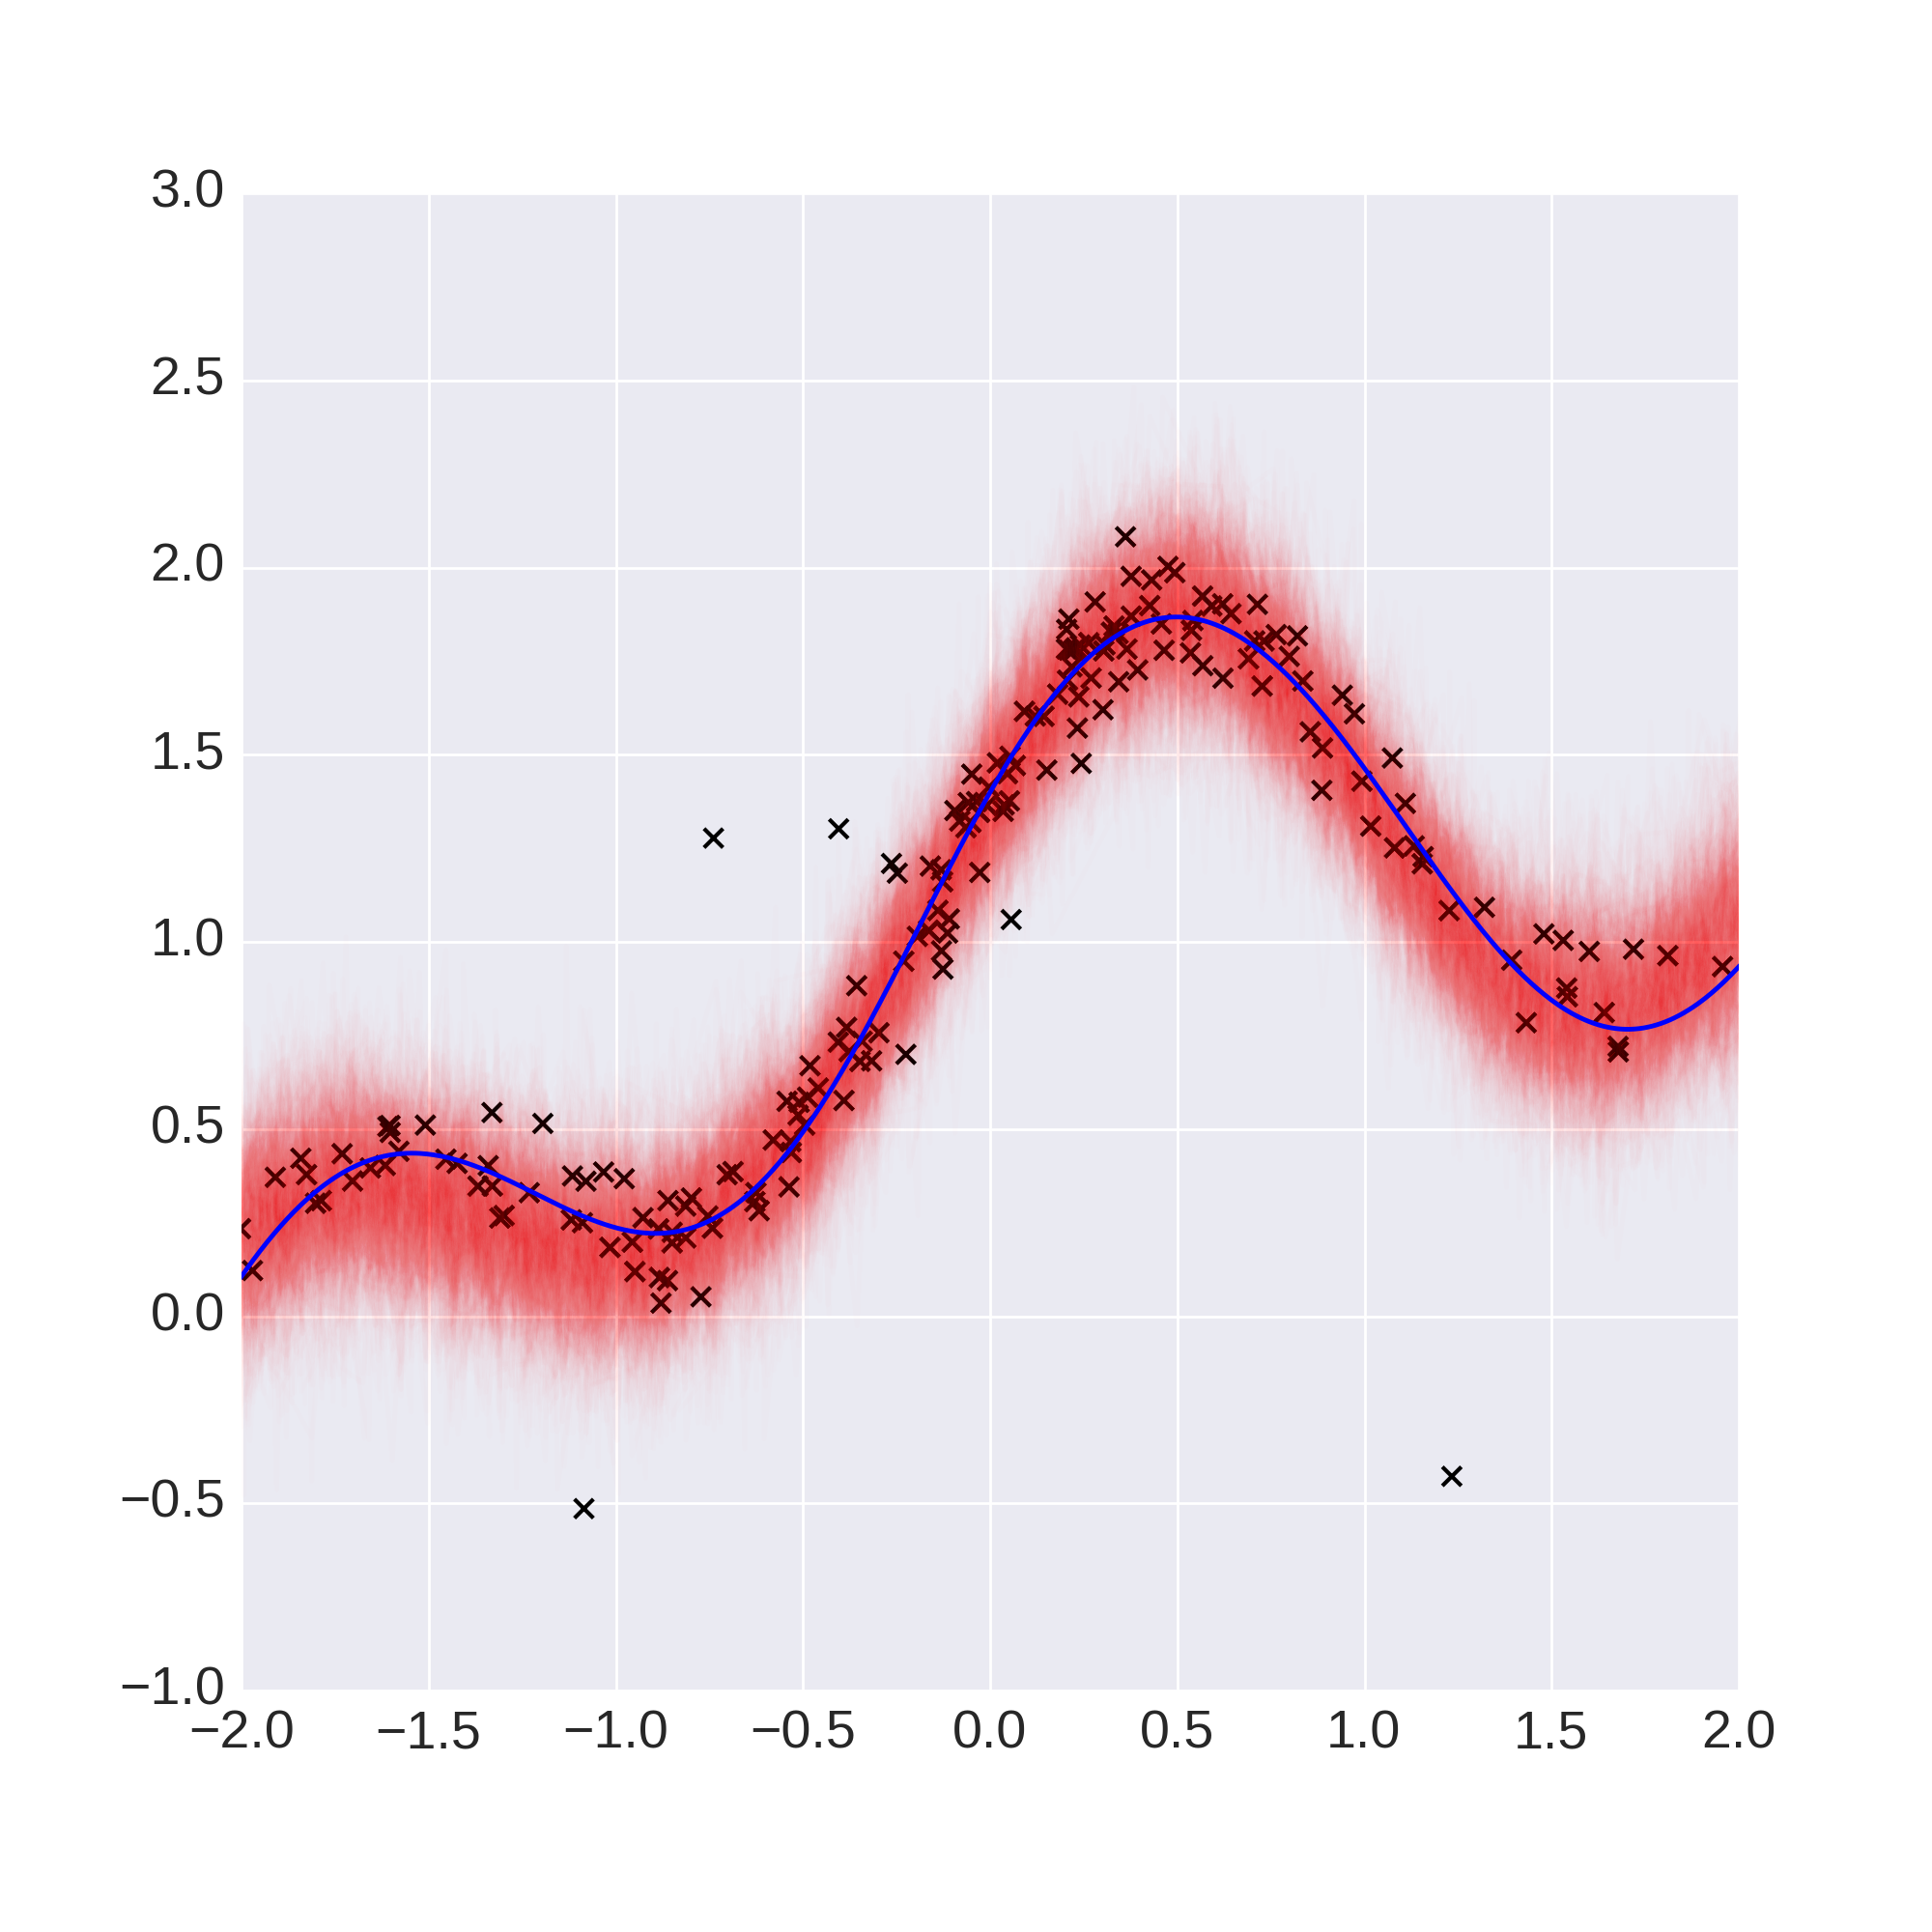
\includegraphics[height=3.9cm]{figs/neal_se_3final.png}
                        \put(-76,24){\color{green} \thicklines \circle{10}}
			\put(-28,26){\color{green} \thicklines  \circle{10}}
			\put(-70,63){\color{green} \thicklines  \circle{10}}
                \caption{Inferred}
                \label{fig:NealAI}
        \end{subfigure}
        		\put(-95,45){\color{green} \thicklines \vector(1,0){20}}
			\put(-96,37){\color{green} \thicklines \vector(1,0){20}}
			\put(-96,78){\color{green} \thicklines \vector(1,0){20}}
    \centering
        \begin{subfigure}[b]{0.24\textwidth} \centering
                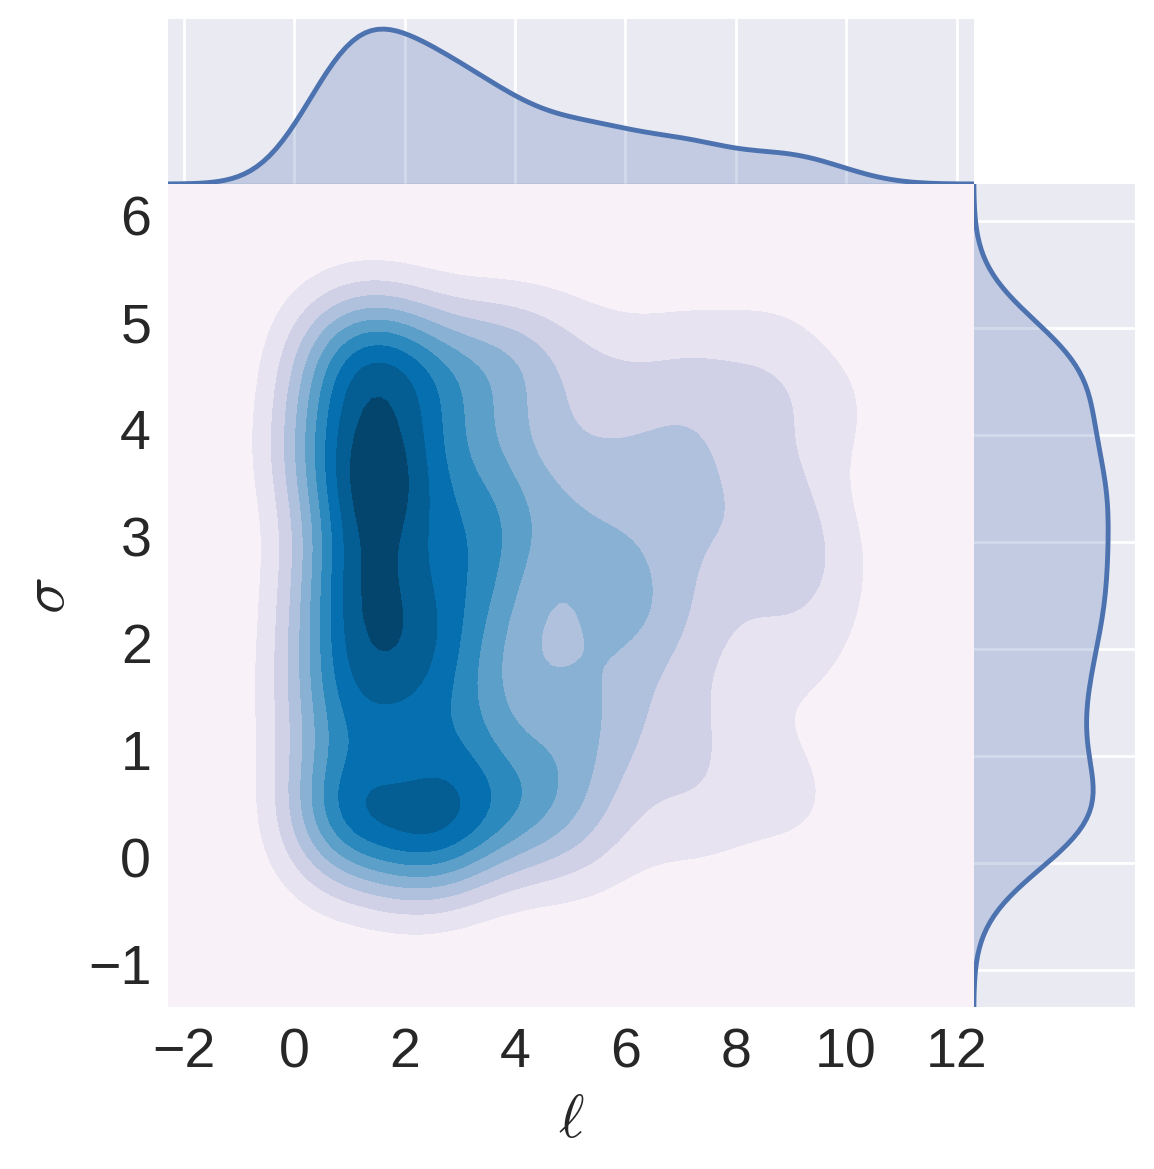
\includegraphics[height=3.5cm]{figs/neal_contour_l_vs_sigma_s__marginal_before.png}
                \caption{Before}
                \label{fig:before}
        \end{subfigure}%
        ~ %add desired spacing between images, e. g. ~, \quad, \qquad, \hfill etc.
          %(or a blank line to force the subfigure onto a new line)
        \begin{subfigure}[b]{0.24\textwidth} \centering
                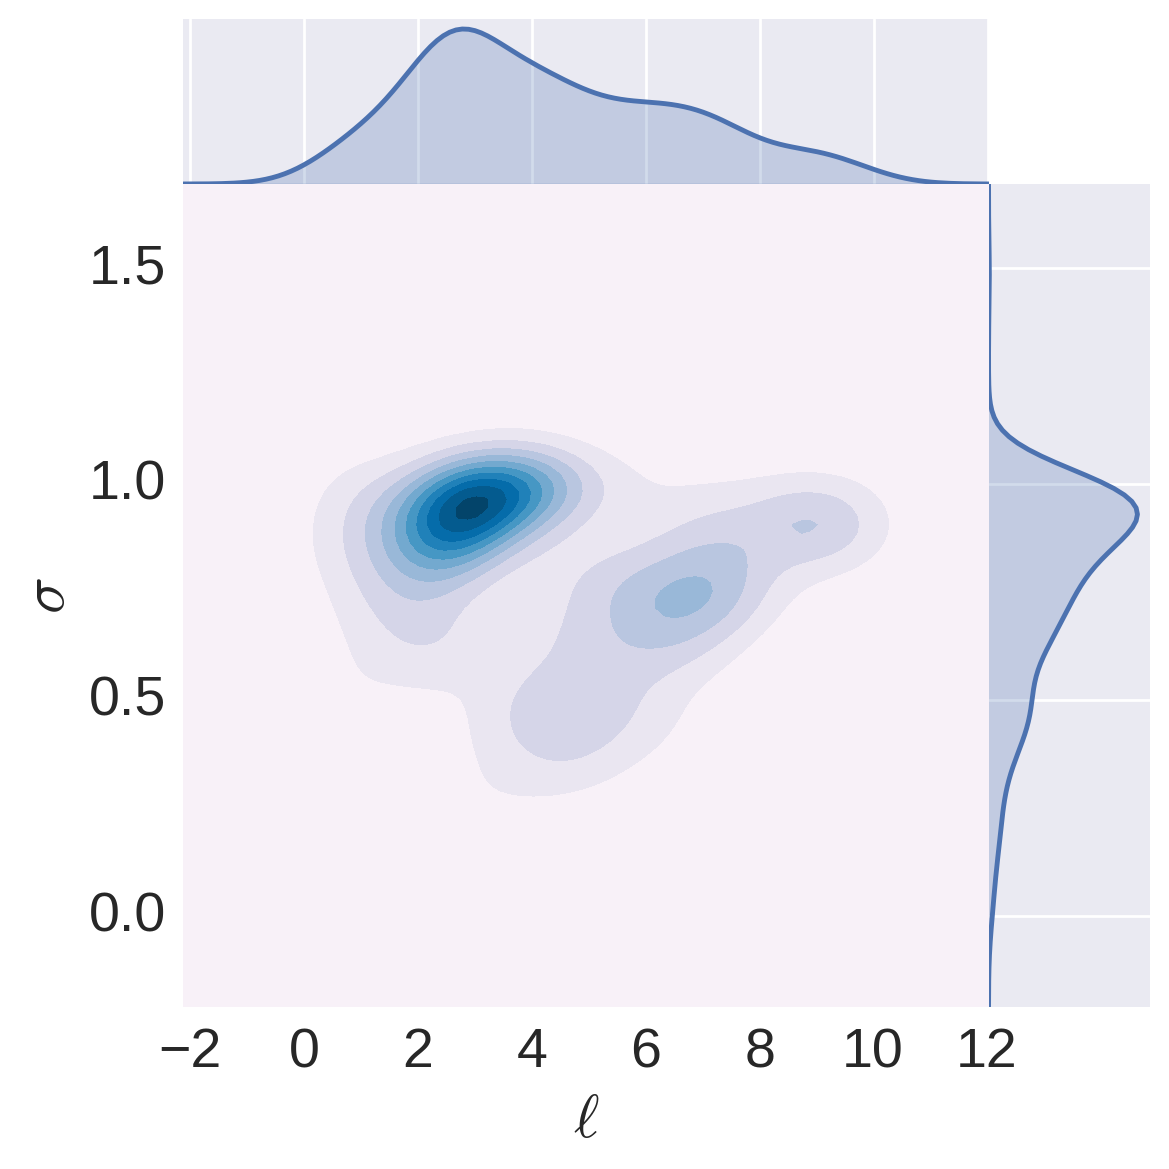
\includegraphics[height=3.5cm]{figs/neal_contour_l_vs_sigma_s__marginal_after.png}
                \caption{After}
                \label{fig:after))}
        \end{subfigure}
        \caption{(a) and (b) show \gpmem\ on Neal's example. Outliers are marked with green circles. After \gpmem\ observes some data-points, an arbitrary smooth trend with a high level of noise is sampled (a). After running inference on the hierarchical system of hyper-parameters we see that the posterior reflects the actual curve well (b). We see that the outliers are rejected. This is partly due to the shift in the hyper-parameters for lengthscale $\ell$ and noise $\sigma$. From a uniform/gamma prior (c) we compute a bimodal posterior (d)}\label{fig:neal}
\end{figure}
\end{comment}
\begin{figure}
\begin{subfigure}[b]{0.49\textwidth}\centering
\begin{tabular}{ll}
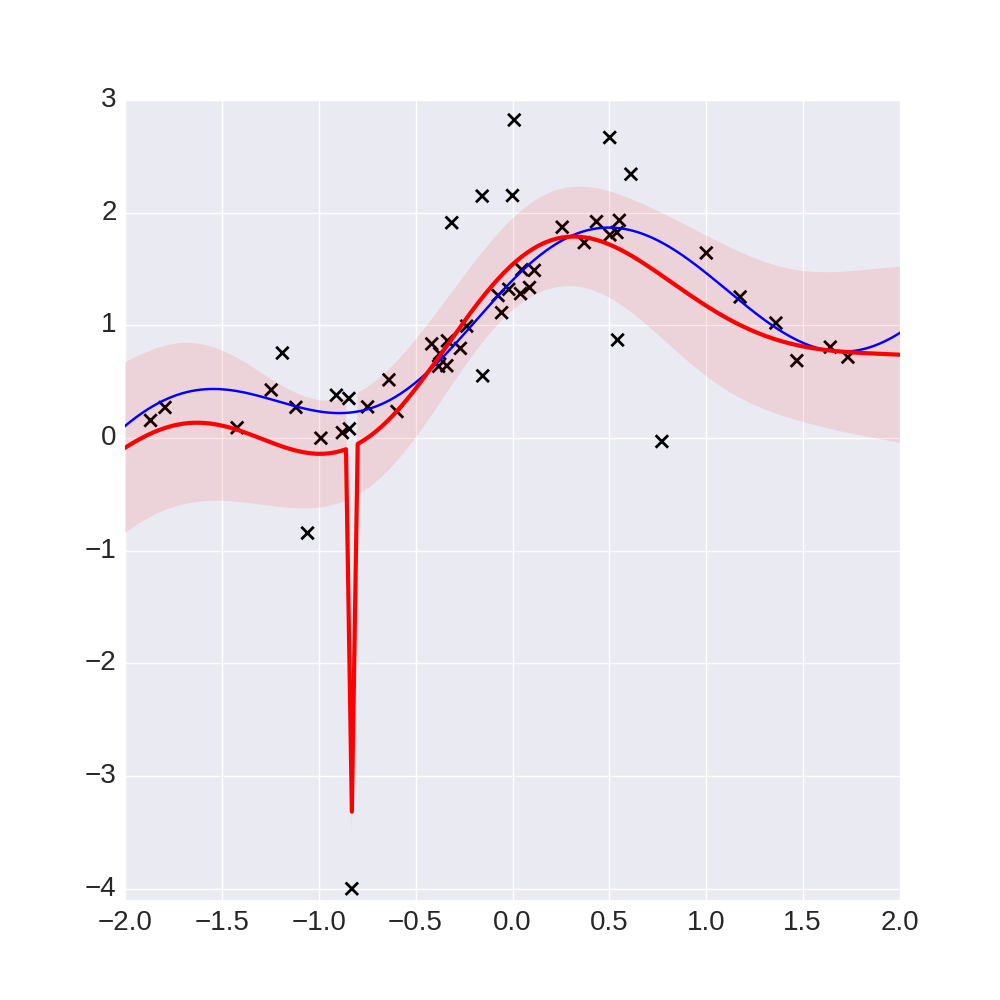
\includegraphics[height=4.5cm]{figs/neal_deterministic.png} &  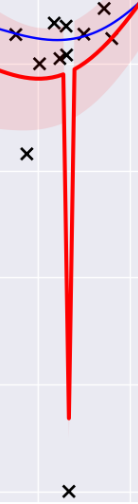
\includegraphics[height=4.5cm]{figs/outlier.png}
\end{tabular}
          \caption{}
          \label{fig:deterministic}
\end{subfigure}          
\begin{subfigure}[b]{0.49\textwidth}\centering
\centering
\begin{tabular}{ll}
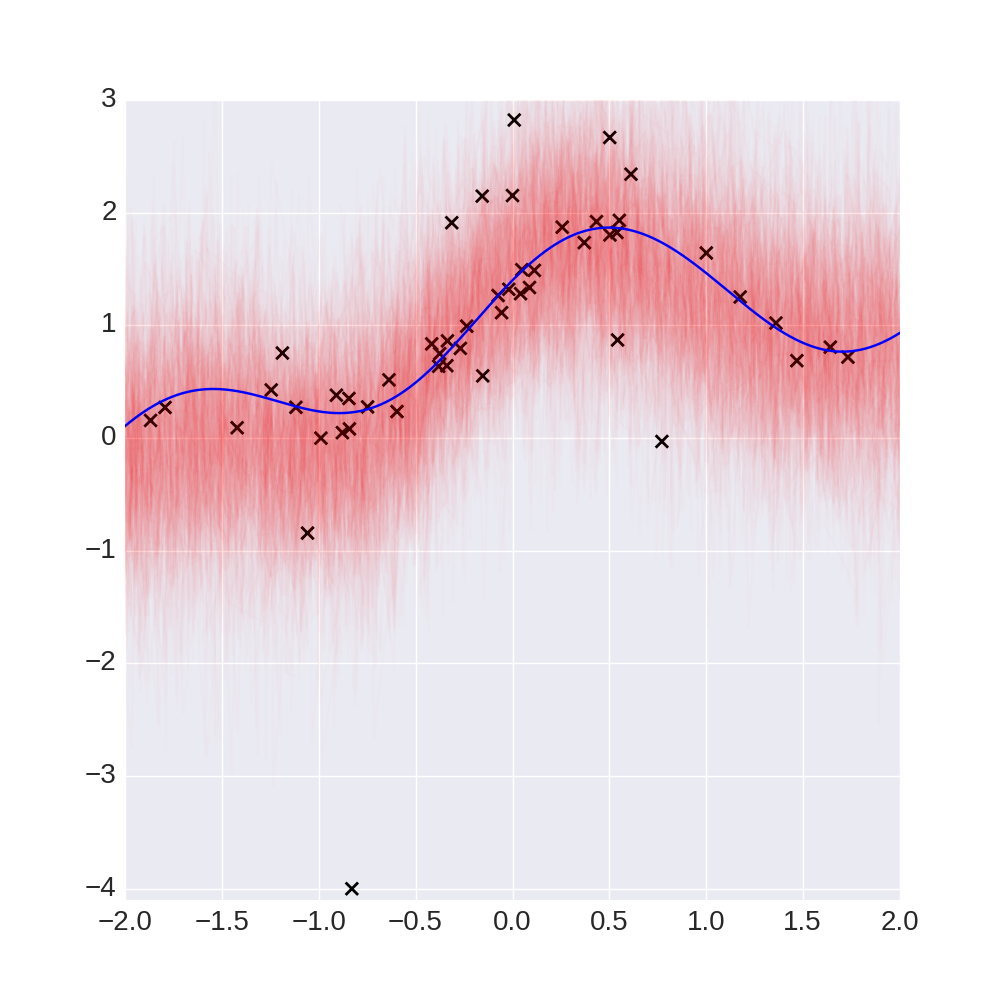
\includegraphics[height=4.5cm]{figs/neal_Bayesian.png} &  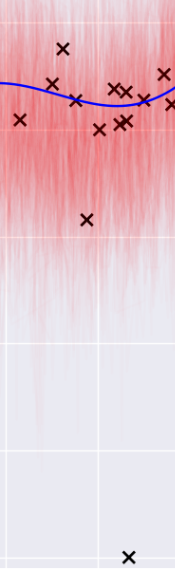
\includegraphics[height=4.5cm]{figs/outlier_Bayesian.png}
\end{tabular}
          \caption{}
          \label{fig:Bayesian}
\end{subfigure}
        		\put(-130,55){\color{green}\thicklines \vector(1,0){80}}
        		\put(-326,55){\color{green}\thicklines \vector(1,0){80}}
			\put(-47,21){\color{green} \thicklines \line(1,0){39}}
			\put(-47,148){\color{green} \thicklines \line(1,0){39}}
		        \put(-47,21){\color{green} \thicklines \line(0,1){127}}
		        \put(-8,21){\color{green} \thicklines \line(0,1){127}}
		        \put(-243,21){\color{green} \thicklines \line(0,1){127}}
		        \put(-206,21){\color{green} \thicklines \line(0,1){127}}
		        \put(-243,21){\color{green} \thicklines \line(1,0){37}}
			\put(-243,148){\color{green} \thicklines \line(1,0){37}}
\caption{(a) a shows deterministic inferece, that is optimization for an example of Neals synthetic function with an extreme outlier (green).}\label{fig:neal}
\end{figure}


We illustrate the hyper-parameters by showing a comparison between $\sigma$ (Fig. \ref{fig:neal}). We see that \gpmem\ learns the posterior distribution well, the posterior even exhibits a bimodal histogram when sampling $\sigma$ 100 times reflecting the two modes of data generation, that is normal noise and outliers. 

\begin{minipage}{\linewidth}
\belowcaptionskip=-10pt
\begin{lstlisting}[frame=single,mathescape,label=alg:gphierarch,basicstyle=\selectfont\ttfamily,numbers=none]
/// SETTING UP THE MODEL
assume alpha_sf = tag(quote(hyperhyper), 0, gamma(7, 1))
assume beta_sf = tag(quote(hyperhyper), 1, gamma(7, 1))
assume alpha_l = tag(quote(hyperhyper), 2, gamma(7, 1))
assume beta_l = tag(quote(hyperhyper), 3, gamma(7, 1))

// Parameters of the covariance function
assume sf = tag(quote(hyper), 0, gamma(alpha_sf, beta_sf)))
assume l = tag(quote(hyper), 1, gamma(alpha_l, beta_l)))
assume sigma = tag(quote(hyper), 2, uniform_continuous(0, 2)) 

// The covariance function
assume se = make_squaredexp(sf, l)
assume wn = make_whitenoise(sigma)
assume composite_covariance = add_funcs(se, wn)

/// PERFORMING INFERENCE
// Create a prober and emulator using gpmem
assume f_restr = get_neal_blackbox()
assume (f_compute, f_emu) = gpmem(f_restr, composite_covariance)

// Probe all data points
predict mapv(f_compute, get_neal_data_xs())

// Infer hypers and hyperhypers
infer repeat(100, do(
    mh(quote(hyperhyper), one, 2),
    mh(quote(hyper), one, 1)))

\end{lstlisting}
\end{minipage}



